\documentclass[11pt]{article}
\usepackage[utf8]{inputenc}
\usepackage[T1]{fontenc}
\usepackage{amsmath}
\usepackage{amsfonts}
\usepackage{amssymb}
\usepackage[version=4]{mhchem}
\usepackage{stmaryrd}
\usepackage{graphicx}
\usepackage[export]{adjustbox}
\graphicspath{ {./images/} }

\begin{document}
\section*{Reading}
Forward Contracts on Assets with Benefits and Costs of Carry

This section discusses the economic benefits and costs of carrying or holding a cash position versus holding a forward position and the implication of those benefits and costs for the pricing of forward contracts. The section moves the focus from financial assets toward physical assets such as commodities.

\section*{The Benefits and Costs of Carry}
In the context of forward contracts, a cost of carry (or carrying cost) is any direct financial difference between maintaining a position in the cash market and maintaining a position in the forward market. For example, being physically long wheat requires storage (and generates storage costs), whereas being long a forward contract on wheat does not require physical storage.

Cost-of-carry models use projections of carrying costs and benefits to value derivatives such as forward contracts. The modeling approach is to identify two strategies that have identical payoffs (cash market vs. forward market) and attribute differences in current prices to differences in the costs of carrying each strategy. A cost-of-carry model assumes that in an informationally efficient market, when two positions converge to an equivalent value at some point in the future, any differences in their current values will be determined exactly by the differences in their carrying costs (and benefits).

The following table lists the categories of carrying costs and benefits for real (physical) assets and for financial assets.

\begin{center}
\begin{tabular}{|lll|}
\hline
\multicolumn{2}{c|}{Benefits and Costs of Direct Ownership} &  \\
\hline
\multicolumn{1}{|c|}{Real Assets} & Financial Assets &  \\
\hline
Benefits & Convenience $(y)$ & Dividends + Coupons $(d)$ \\
Costs & Interest $(r)+$ Storage $(c)$ & Interest $(r)+$ Custody (zero) \\
\hline
\end{tabular}
\end{center}

There are two key entries in the above table that warrant special consideration: convenience and storage. Convenience, expressed in a rate as convenience yield ( $y$ ), is the economic benefit that the holder of a physical inventory (e.g., a commodity) receives from directly holding the inventory rather than having a long position in a forward contract on the physical assets.

Gold provides a vivid example of convenience yield. For a firm that uses gold in its production process, such as a jewelry manufacturer, an inventory of gold helps protect it from supply disruptions. A forward contract on gold might offer protection from changes in the market price of gold, but ultimately the jewelry manufacturer needs physical inventory to ensure that production will not be disrupted. For another holder of gold, the convenience yield of the gold inventory may be the value to the holder of having an emergency asset that might offer exchange value during even the most terrible times for the economy. In both cases, physical ownership of the asset may be viewed as more valuable than synthetic ownership (i.e., ownership through a forward contract to take delivery), since the physical ownership provides a more immediate and certain ability to use the asset for an intended purpose.

Convenience yield serves the holder of a nonfinancial commodity in the same direction that the dividend yield serves the owner of a financial asset; therefore, dividends and convenience yield both enter pricing models with the same sign (a negative sign to denote that a benefit is the same as a negative cost). However, a key distinction is that different market participants have different convenience yields for a given physical asset that vary based on their individual circumstances, whereas each holder of a particular financial asset receives the same dividends (or interest). For example, natural gas can have substantially different convenience yields-which in turn can vary based on seasons and weather (due to its use as a heating fuel). This is in contrast to the benefits of financial assets shown in the above exhibit (dividends and other distributions), which tend to have clear and somewhat unanimously perceived economic values.

Storage costs of physical assets (e.g., commodities) involve such expenditures as warehouse fees, insurance, transportation, and spoilage. Storage costs are of the sign opposite to that of dividends, since they are costs of holding the underlying asset rather than benefits. Accordingly, the storage costs expressed as a continuous rate, $c$, can be an important determinant in the pricing relationship. Storage costs enter using the same sign as $r$, the opportunity cost of capital, since both reflect costs of ownership of a physical commodity. In fact, the financing cost, $r$, of holding the physical commodity can be included as part of $c$. However, storage costs for physical assets such as natural gas can vary substantially between market participants. This is in contrast to the opportunity cost of capital $(r)$ of both financial assets and physical assets, which tend to have clear and somewhat unanimously perceived economic values.

Note that the above exhibit depicts carrying costs of holding physical assets. The storage costs are positive carrying costs that, everything else equal, make holding a physical inventory unattractive. Forward contracts on the same commodity do not have storage costs. Therefore the storage costs of physical assets, $c$, make forward contracts more attractive than physical inventories, everything else equal. Of course everything else is usually not equal. Physical inventories typically offer convenience yield, $y$, which is an attractive feature that forward contracts do not offer. This explains why $c-y$ must appear in a model of the relative values of forward prices and spot prices on commodities.

\section*{The Forward Price of a Commodity}
Equation 4 in the lesson Forward Contracts on Equities provides the formula for a forward price on a financial asset based on the spot price of the underlying asset that uses two variables: the riskless interest rate and the underlying asset's dividend yield. The right side of the above exhibit lists these two variables as costs (the riskless rate reflects the cost of carry of a cash position) and benefits (the dividend yield is a benefit of a cash position), respectively. Replacing the costs and benefits of carrying a cash position of a financial asset with the costs and benefits of carrying physical inventory (the left side of Benefits and Costs of Direct Ownership) generates the formula for a forward contract on a commodity in Equation 1.


\begin{equation*}
F_{T} \leq P_{0} e^{(r+c-y) T} \tag{1}
\end{equation*}


where $r$ is the spot interest rate corresponding to a time to maturity of $T$ years, $c$ is the commodity's storage cost, and $y$ is the commodity's convenience yields, all expressed as continuously compounded annual rates.

Note that the relationship is expressed as an inequality in Equation 1 in contrast to the equality relationship for a financial asset in Equation 4 in the lesson Forward Contracts on Equities. This is due to potential problems with short-selling a physical asset.

Dividing through Equation 1 by $P_{0}$, assuming that it is an equality, and taking the logarithm of each side and factoring, generates:

Implied growth rate of forward over spot $=r+c-y$

In words, the price ratio of the forward price to the spot price (expressed as a continuously compounded rate) is the sum of the two benefits to having the forward position (avoiding the carrying costs of a physical inventory including financing costs and storage costs) minus the cost to an investor of using a forward contract rather than a physical inventory (losing the convenience yield).

\section*{Four Factors Differentiating Forward Pricing on Financial and Physical Assets}
Previous sections detailed the arbitrage-free price of a forward contract on a financial security based on comparing the carrying costs of a spot market transaction with those of a forward market transaction. This section contrasts the determinants of forward prices for financial securities with the determinants of forward prices for commodities.

A central concept in understanding forward contracts is that in the simple case of forward contracts on financial securities, the forward prices of the contracts are driven entirely by spot prices including the level and shape of the term structure of interest rates (and prospective dividend yields). Formulas for the forward prices therefore contain current market values, such as spot prices, and current rates, such as risk-free interest rates and dividend yields. Arbitrageurs able to hedge either long or short positions in the forward contracts force the relationship to hold.

Forward prices on financial assets do not reveal information on future price changes beyond the information already contained in spot prices. For example, it is a mistake to interpret the shape of forward interest rate curves as containing information beyond what is in the term structure of spot rates because there is a one-toone relationship between the two structures. Similarly, expected spot prices do not drive the spread between forward prices and spot prices for financial assets.

However, forward prices on physical assets are different. Many alternative investment strategies involve forward contracts (or futures contracts, detailed later in this session) on assets other than financial securities, in particular, commodities. Commodity forward prices and the term structure of forward prices on commodities often do not adhere to a strict cost-of-carry relationship for several reasons. The forward structure's shape for commodities and other real assets can be driven by at least four additional factors: (1) forecasts of supply and demand changes, (2) storage cost differentials, (3) convenience yield differentials, and (4) difficulties with short selling.

\section*{Challenges Involving Measuring Storage Costs and Convenience Yields}
If $c$ and $y$ are observable marketwide values and if physical assets can be limitlessly short sold, forward contracts would be strictly priced according to Equation 1 in perfect and competitive markets. However, storage costs and convenience yields of physical assets have a very important difference relative to the dividend yield on financial assets: Storage costs and convenience yield can be expected to vary with location and market participants, as well as with supply and demand.

For example, storage costs for natural gas are seasonal on account of increased winter demand. Storage costs for agricultural and other products can be seasonal as well, relating to harvest times. Since anticipated supply and demand factors can cause storage costs to vary through time, the pricing relationships between forward contracts of different delivery dates (i.e., the term structure of forward prices) can reflect anticipated supply and demand. Further, storage costs vary between participants.

From the perspective of an individual entity, Equation 1 can be viewed as associating the entity's storage costs and convenience yields with the relative values of the spot and forward prices of the commodity. From the marketwide perspective, Equation 1 can be viewed as relating the relationship between the forward and spot prices of a commodity to the spread between the storage costs and convenience yield $(c-y)$ of the marginal market participant. The marginal market participant to a derivative contract is any entity with individual costs and benefits that make the entity indifferent between physical positions and synthetic positions.

As in the case of storage costs, convenience yield can be expected to vary through time and across market participants and locations. One entity might perceive tremendous advantage from having a large supply of a commodity in inventory (i.e., being able to meet unexpected demand or unforeseen supply disruptions), and another entity might perceive little advantage.

The convenience yield of a particular commodity to a consumer or a producer would typically be much higher when there is a general shortage of the commodity (i.e., low inventories). Thus, a manufacturer of silver-plated products would derive more convenience yield from holding an inventory of silver at a time when silver is scarce and the danger of being unable to obtain adequate silver supplies is higher.

The potential for storage costs and convenience yield to vary through time and have predictable changes through time adds to the reasons that the term structure of forward prices will not be monotonically upward sloping or downward sloping as depicted in the exhibit Forward Term Structures in the previous lesson, Forward Contracts on Equities. In the case of a commodity such as natural gas, the next exhibit demonstrates a pronounced wave pattern of the term structure of forward prices to reflect the anticipated effects of seasonal demand on storage costs and convenience yield.

\begin{center}
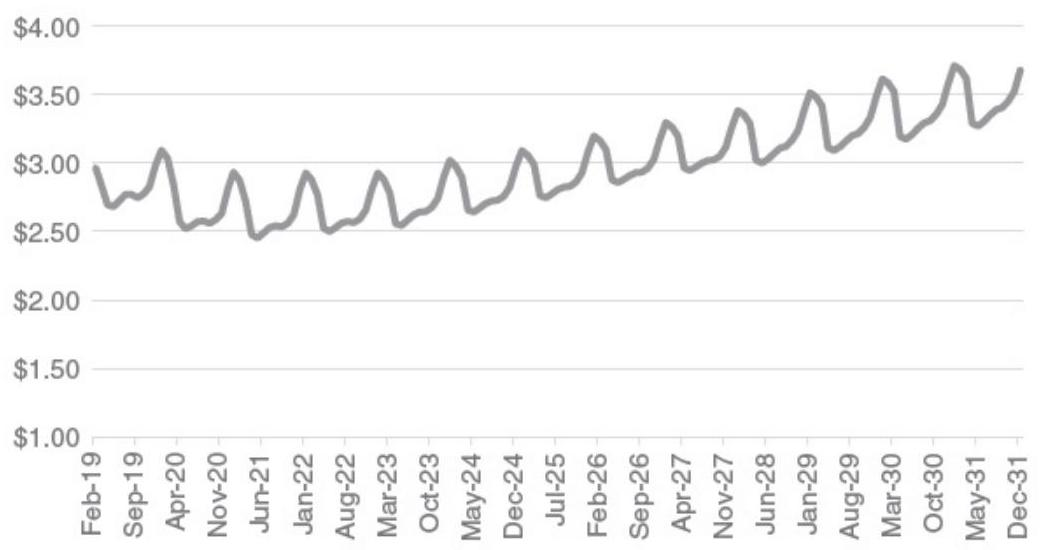
\includegraphics[max width=\textwidth]{2024_04_10_524707c94c7a5febe5e0g-4}
\end{center}

\section*{Term Structure of Natural Gas Futures Closing Prices}
Source: Data from Bloomberg.

Further, the idea that the slope and shape of the term structure of forward prices depends not only on observed values (e.g., the riskless rates and dividend yields) but also on predictions of supply and demand means that superior supply and demand forecasting may offer superior returns to market participants better able to predict supply and demand. In other words, market participants can speculate on the shapes and slopes of the term structure of forward prices and may consistently generate superior returns if their abilities to forecast supply and demand (and, to a lesser extent, storage costs and convenience yields) are superior.

\section*{Short Selling of Physical Assets}
The lesson, Short Selling discussed short-selling of financial assets, wherein there is a well-organized market for the lending and borrowing of stocks and bonds. Previous sections in this session have relied on the actions of hypothetical arbitrageurs to force specific relations between forward prices and spot prices based on carrying costs and benefits. Specifically, Equation 4 in the lesson Forward Contracts on Equities is premised on the ability of arbitrageurs to establish long positions in a forward contract to hedge a short position in its underlying asset and establish short positions in a forward contract to hedge a long position in its underlying asset because the asset is a financial asset.

But developed markets for lending physical assets such as commodities do not exist to the extent that such markets exist for lending financial assets. Without commodity lending, the arbitrageurs cannot short-sell commodities to form a hedge against a long position in a forward contract. This inability to hedge a long position in a forward contract inhibits the ability of arbitrageurs to take on long positions in a forward contract, thereby preventing arbitrage from driving underpriced forward prices to their theoretical values. As a result, Equation 1 expresses the forward price as being less than or equal to its theoretical value in the case of a forward contract on a physical asset when that physical asset (the underlying asset) cannot be shorted.

\section*{Forward Contracts with Nonzero Market Value}
The material on forward contracts in the previous sections has focused on the forward price (or rate) that is set at the initiation of the forward contract under the assumption that the contract is initiated with a market value of zero (i.e., no cash is exchanged between the parties to initiate the contract). It is possible that the long and short sides of the contract agreed to a forward price that caused the contract to have a nonzero initial value, especially if one of the sides of the contract made an immediate payment to the other side to initiate the contract. Further, it is expected that forward contracts will take on various positive or negative values to each side of the contract after the contract is initiated as the market price (or rate) of the contract's underlying asset (or rate) moves up or down.

Equation 2 expresses the value to the long side of a forward contract under the assumption that the underlying asset can be readily short-sold.

Value of long position in forward contract at time $t=P_{t} e^{(r+c-y)(T-t)}-F_{0}$

where $P_{t}$ is the price of the contract's underlying (deliverable) asset at time $T, F_{0}$ is the forward price of the contract (set at the contract's initiation to generate a zero value to the contract), and other variables are as previously defined (included at their time $T$ values). The value to the short side has the opposite sign in a perfect market. Note that at $t=T$, the value of the forward contract is $P_{t}-F_{0}$, which is the cash settlement to (from) the long side from (to) the short side when $P_{t}-F_{0}$ is positive (negative).


\end{document}